 \chapter{Proponowany model zjawiska}

\section{Cele modelu}
Celem modelu jest zasymulowanie rozwoju populacji zwierząt. Stworzony przez nas program pozwala na zasymulowanie populacji modelu drapieżnik-ofiara w postaci :
\begin{itemize}
	\item jednego gatunku ofiary i  jednego gatunku drapieżnika, który żywi się ofiarą
	\item jednego gatunku ofiary,  drapieżnika żywiącego się ofiarami oraz drapieżnik drugiego stopnia żywiącego się zarówno ofiarami jak i drapieżnikami, lecz preferującemu drapieżniki.
\end{itemize}
 
Zwierzęta mogą poruszać się po zadanym obszarze nie opuszczając go. 

Gdy osoba rozpocznie symulacje może na bieżąco wyświetlać informacje na temat liczby iteracji, ilości populacji każdego z gatunków. Dodatkowo przedstawiony jest widok mapy migracji zwierząt.

System modeluje zachowanie 

\section{Działanie algorytmu} 
W pierwszym etapie działania programu generowanie są populacje zadanych gatunków. Stworzone populacje są rozmieszczane losowo na mapie w ilości uzależnionej od zadanych przez nas współczynników. Następnie na każdym z pól tworzona jest ilość pożywienia dla ofiar, czyli rośliny. 

Po inicjalizacji modelu rozpoczyna się główna część symulacji. W każdej iteracji każde zwierzę obejmuje jakąś strategię działania.
\begin{enumerate}
\item Wspólne na wszystkich zwierząt
	\begin{itemize}
		\item Kopulacja
		\item Wydawanie na świat potomstwa
	\end{itemize}
\item Dla ofiar
	\begin{itemize}
		\item Poszukiwanie i spożywanie roślin
		\item Ucieczka przed drapieżnikami
		\item Odpoczynek
	\end{itemize}
\item Dla drapieżników
	\begin{itemize}
		\item Polowanie na ofiary
		\item Ucieczka przed drapieżnikami drugiego stopnia
	\end{itemize}
\item Dla drapieżników drugiego stopnia
	\begin{itemize}
		\item Polowanie na ofiary i drapieżników
	\end{itemize}
\end{enumerate}

Poszczególne zachowania uzależnione są od aktualnego stanu danego zwierzęcia oraz jego otoczenia.

\begin{enumerate}
\item Wspólne strategie zwierząt
	\begin{itemize}
		\item Jeżeli samica jest w kluczowym stadium ciąży musi wydać na świat potomstwo.
		\item Jeżeli zwierzę jest zagrożone stara się uciec.
		\item Jeżeli współczynnik głodu jest krytyczny ofiara usiłuje zdobyć pokarm.
		\item Jeżeli współczynnik pożądania seksualnego jest krytyczny i osobnik jest wystarczająco dojrzały rozmnaża się z drugim przedstawicielem swojego gatunku przeciwnej płci na danym polu lub szuka partnera w swojej okolicy.
		\item Jeżeli zwierze ma wszystkie współczynniki w normie, odpoczywa.
	\end{itemize}
	
\item Szczególne dla ofiary
	\begin{itemize}
		\item Jeżeli na polu jest drapieżnik, który poluje na ofiarę stara się uciec z danego pola
		\item Jeżeli współczynnik głodu jest krytyczny ofiara żywi się pokarmem na aktualnym polu lub jeśli pole jest pozbawione roślin ofiara szuka ich w swoim najbliższym otoczeniu.
	\end{itemize}
	
\item Dla drapieżnika
	\begin{itemize}
		\item Jeżeli na jego polu jest drapieżnik drugiego stopnia, drapieżnik stara się przemieścić w dogodniejsze dla siebie miejsce
		\item Jeżeli współczynnik głodu jest krytyczny drapieżnik poluje na ofiarę znajdującą się na jego polu lub szuka jej w swoim najbliższym otoczeniu.
	\end{itemize}
	
\item Dla drapieżnika drugiego poziomu
	\begin{itemize}
		\item Jeżeli współczynnik głodu jest krytyczny drapieżnik drugiego stopnia w pierwszej kolejności stara się upolować drapieżnika, który jest preferowanym gatunkiem. W razie jego braku poluje na przedstawiciela gatunku reprezentowanego przez ofiarę.
	\end{itemize}
\end{enumerate}

Dodatkowo w celu organiczna ekspansji populacji ofiar liczba roślin na mapie jest ograniczona przez współczynniki regeneracji roślin po każdej iteracji. Po każdej iteracji zwiększany jest wskaźnik głodu dla każdego zwierzęcia oraz pożądania seksualnego dla dojrzałych osobników. Zwierzę po spożyciu pokarmów otrzymuje wartość energetyczną zjadanego pokarmu, która obniżka wskaźnik głodu.

\section{Symulacja zjawiska}

\subsection{Narzędzi}
Na potrzeby symulacji została stworzona aplikacja okienkowa, która wizualizuje efekty działania programu.
Do zaimplementowania programu posłużyliśmy się językiem Java, a do wyświetlenia danych użyliśmy biblioteki graficznej JavaFX.
\subsection{Aplikacja}
Poniżej przedstawiamy kilka zrzutów ekranu w takcie działa aplikacji.
\subsubsection{Symulacja dla 2 gatunków}
Poniższe obrazy prezentują zachowanie się aplikacji dla dwóch gatunków zwierząt. Na rysunku \ref{fig:pp1} widać jak ofiary i drapieżniki żyją w pomieszanych stadach (początkowe iteracji), a na rysunku \ref{fig:pp2} widzimy jak uformowały się stada poszczególnych populacji.

\begin{figure}[!htb]
	\centering
	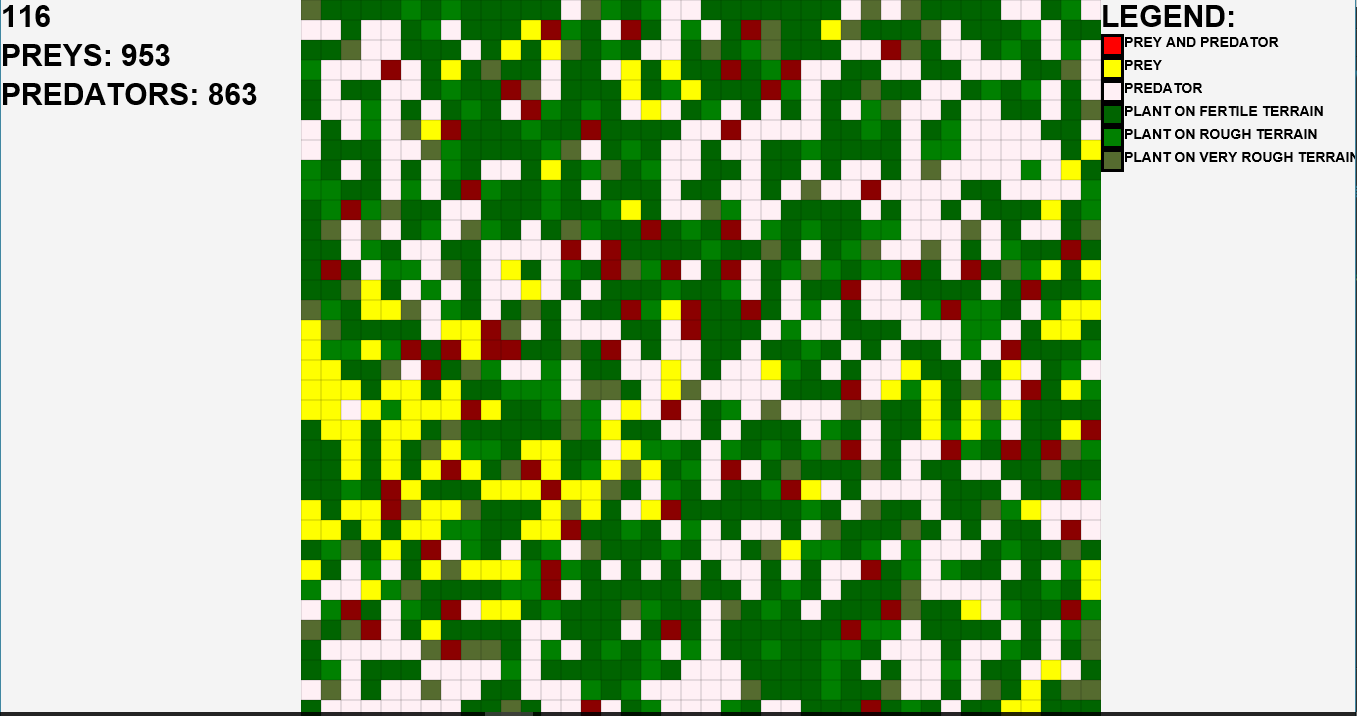
\includegraphics[width=1.1\linewidth]{img/tii1}
	\caption{\label{fig:pp1} }
\end{figure}

\begin{figure}[!htb]
	\centering
	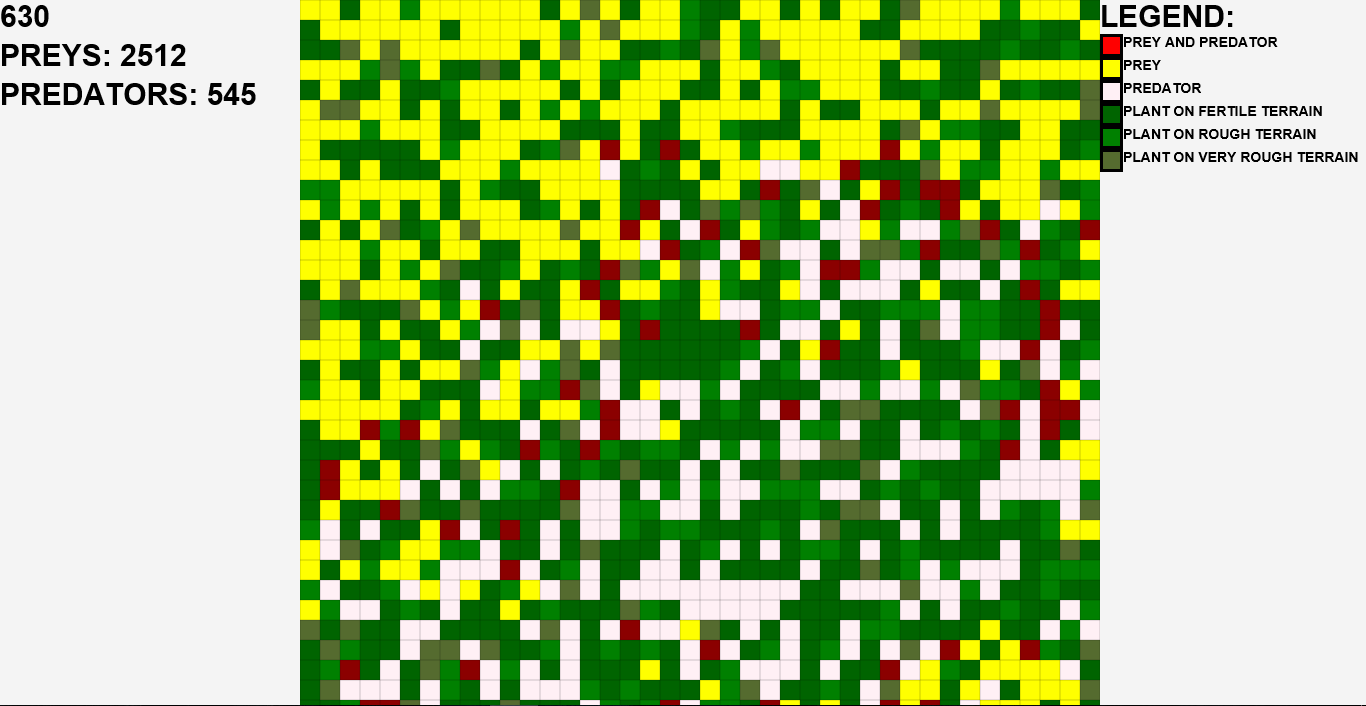
\includegraphics[width=1.1\linewidth]{img/tii2}
	\caption{\label{fig:pp2} }
\end{figure}

\subsubsection{Symulacja dla 3 gatunków}
Poniższe obrazy prezentują zachowanie się aplikacji dla trzech gatunków zwierząt(ofiara, drapieżnik i drapieżnik drugiego stopnia). Na rysunku \ref{fig:pps1} widać jak ofiary i drapieżniki żyją w pomieszanych stadach (początkowe iteracji), a na rysunkach \ref{fig:pps2} \ref{fig:pps3} widzimy jak uformowały się stada poszczególnych populacji.
\begin{figure}[!htb]
	\centering
	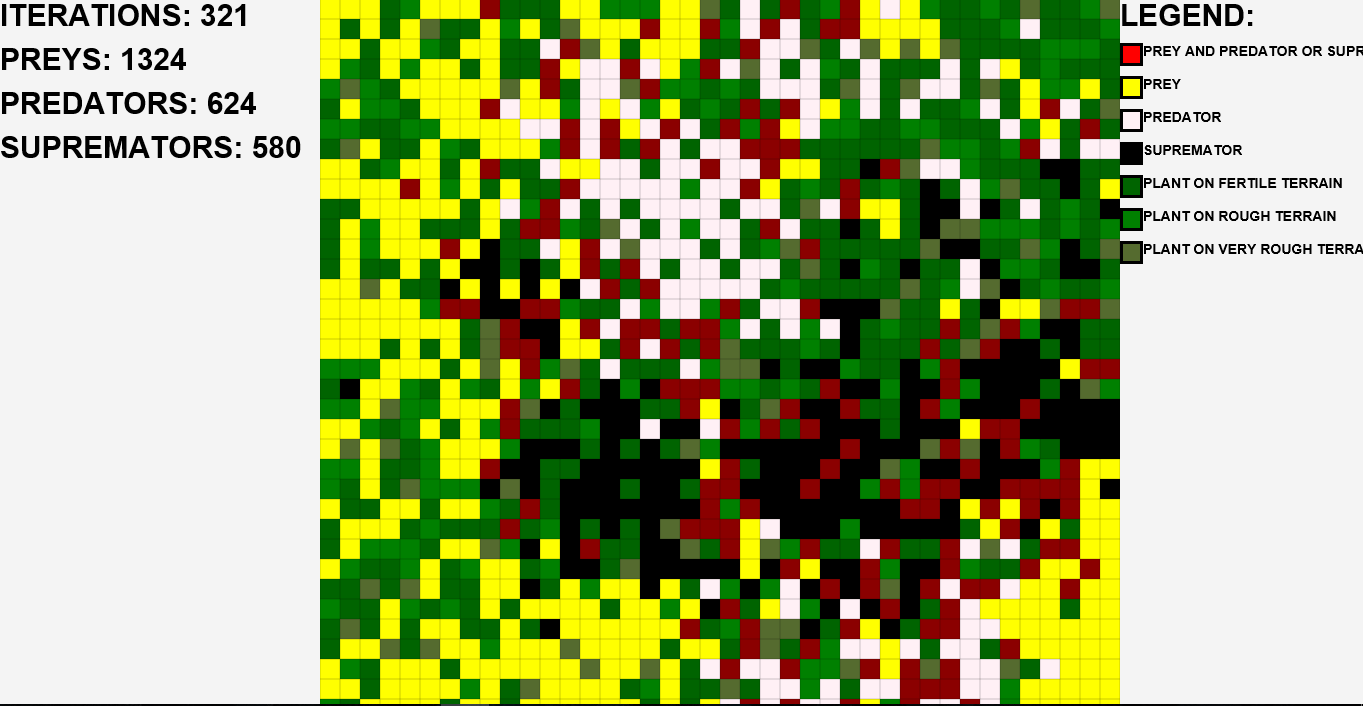
\includegraphics[width=1.1\linewidth]{img/dare}
	\caption{\label{fig:pps1} }
\end{figure}

\begin{figure}[!htb]
	\centering
	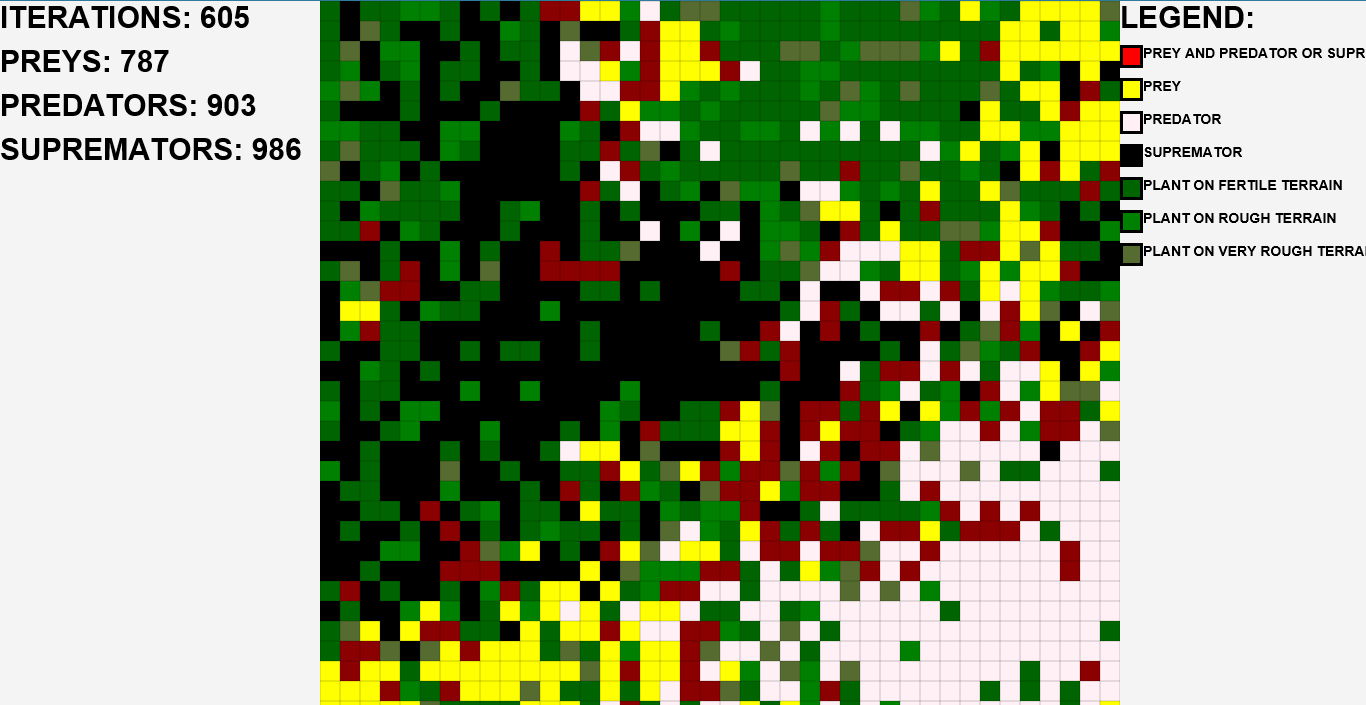
\includegraphics[width=1.1\linewidth]{img/dare2}
	\caption{\label{fig:pps2} }
\end{figure}

\begin{figure}[!htb]
	\centering
	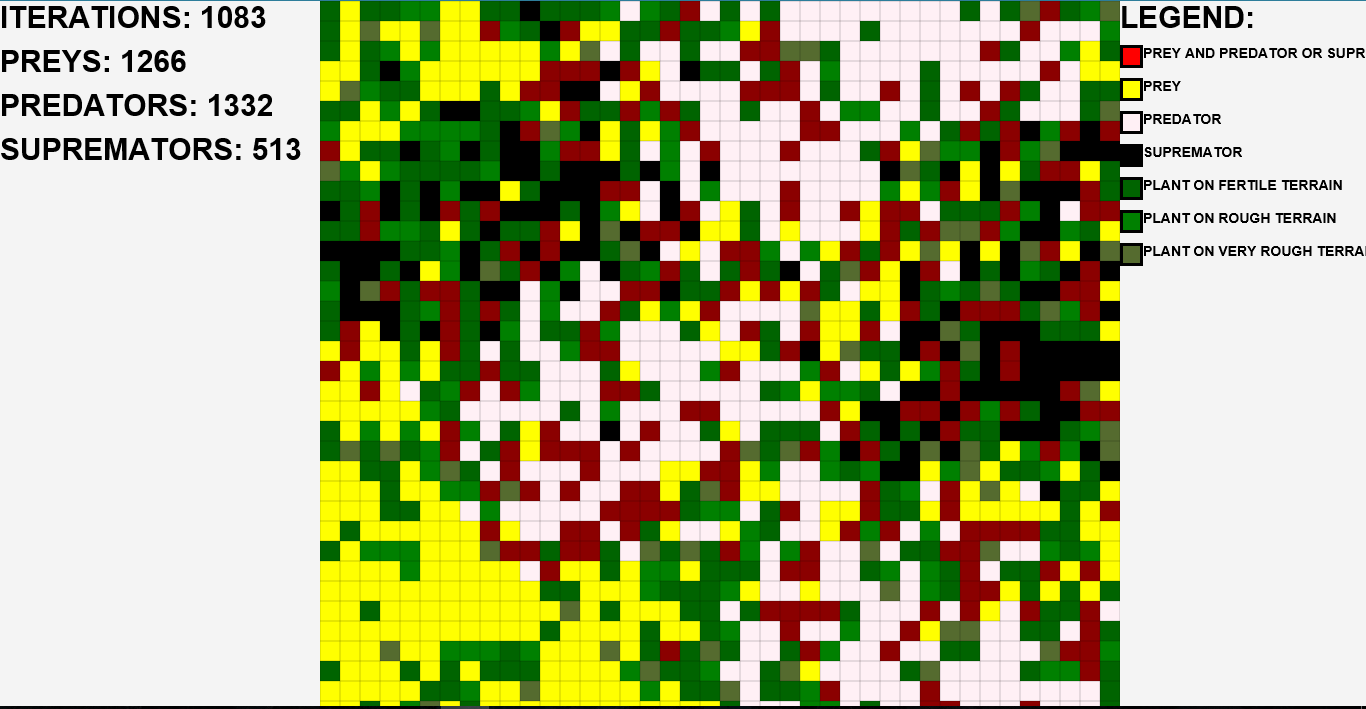
\includegraphics[width=1.1\linewidth]{img/dare3}
	\caption{\label{fig:pps3} }
\end{figure}

 Warto też zwrócić uwagę na to ze życie w większych stadach z dala od swoich ofiar powoduje zagrożenie gatunku i przymus migracji.
 
\newpage
\subsection{Wyniki}

Wyniki kilku symulacji zapisaliśmy do pliku tekstowego, a następnie stworzyliśmy na tej podstawie odpowiednie wykresy. W celu późniejszej możliwości walidacji przyjętego przez nas modelu.
Rysunek 1.1 przestawia wykres zależności ilości drapieżników od ilości ofiar w trakcie próby liczącej 2000 iteracji.
Dodatkowo należy dodać żę wszystkie symulacje uruchamiane były z takimi samymi parametrami, a mimo to otrzymaliśmy inne rezultaty. 
\newpage




\subsubsection{Wyniki dla 2 gatunków- ofiara, drapieżnik}


\begin{figure}[!htb]
	\centering
	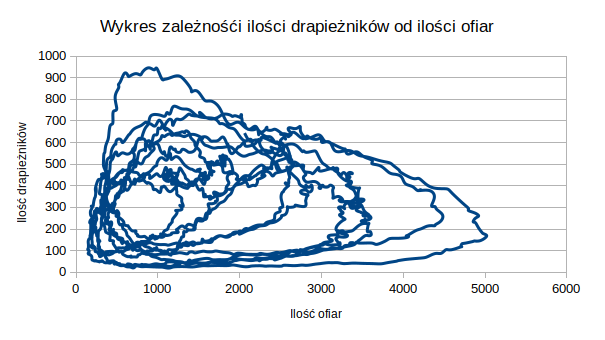
\includegraphics[width=1.1\linewidth]{img/ok11}
	\caption{\label{fig:screen} }
\end{figure}
Powyższy wykres zależności ilość drapieżników od ofiar jest zbliżony do portertu fazowego Lotki-Voltery.
\begin{figure}[!htb]
	\centering
	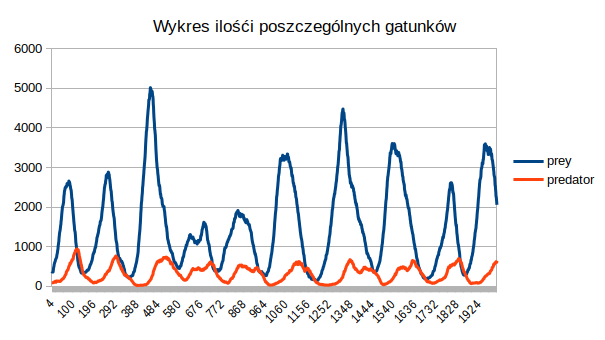
\includegraphics[width=1.1\linewidth]{img/ok1}
	\caption{\label{fig:screen} }
\end{figure}

\begin{figure}[!htb]
	\centering
	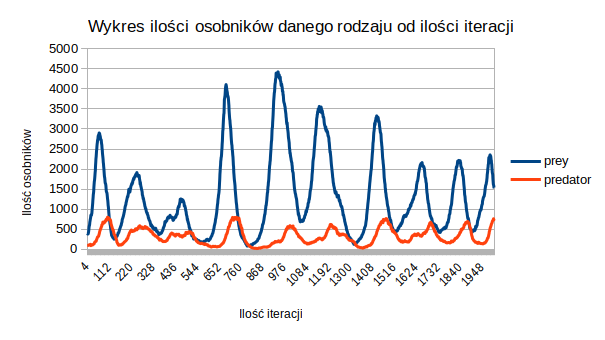
\includegraphics[width=1.1\linewidth]{img/ok2}
	\caption{\label{fig:screen} }
\end{figure}



\begin{figure}[!htb]
	\centering
	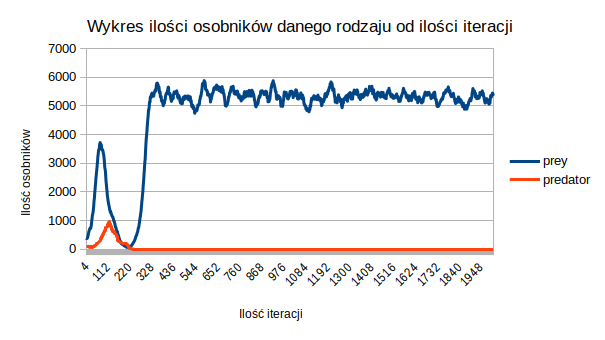
\includegraphics[width=1.1\linewidth]{img/samprey1}
	\caption{\label{fig:screen} }
\end{figure}

\subsubsection{Wyniki dla 3 gatunków- ofiara, drapieżnik i drapieżnik drugiego stopnia}


\begin{figure}[!htb]
	\centering
	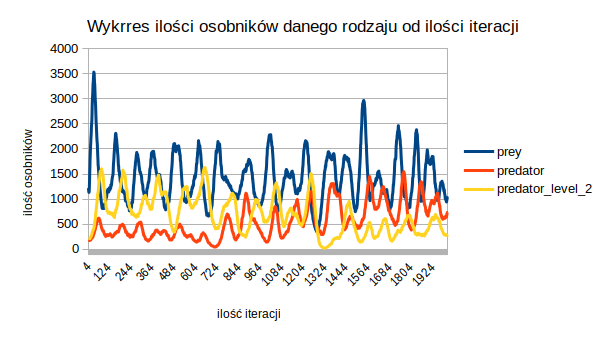
\includegraphics[width=1.1\linewidth]{img/ok3}
	\caption{\label{fig:screen} }
\end{figure}
\begin{figure}[!htb]
	\centering
	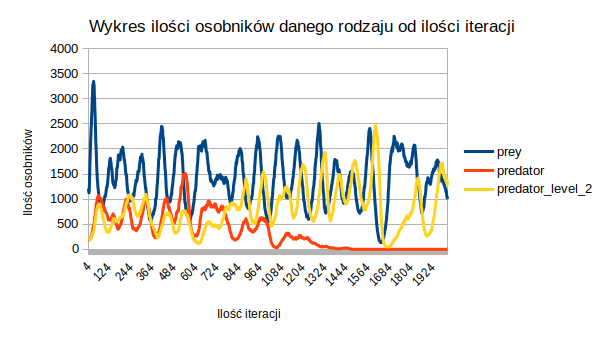
\includegraphics[width=1.1\linewidth]{img/ok4}
	\caption{\label{fig:screen} }
\end{figure}

\begin{figure}[!htb]
	\centering
	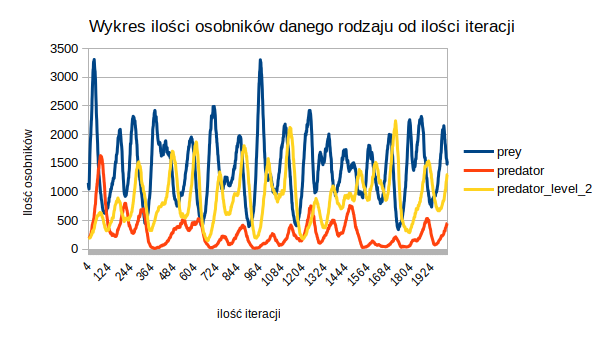
\includegraphics[width=1.1\linewidth]{img/ok5}
	\caption{\label{fig:screen} }
\end{figure}

\section{Wnioski}

Podstawowym wnioskiem jaki zauważyliśmy podczas tworzenia projektu jest to że część współczynników ma ogromny wpływ na działanie i resultat symulacji, a część znikomy. Głównymi współczynnikami naszej symulacją są:
\begin{itemize}
	\item szansa upolowania ofiary
	\item maksymalna możliwa do pokonania odległość w trakcie jednej iteracji
	\item przyrost współczynnika głodu 
\end{itemize}
 Wpływ na wyniki ma też miejsce ulokowania poszczególnych gatunków. Jeżeli już na samym początku drapieżniki otaczają populacje ofiar to  oba gatunki wyginął po upływie kilkunastu iteracji.  

W sytuacji kiedy nasza populacja ofiar w początkowej fazie działania apliakcji da się zagonić w krawędzie, dostępnego pola, podczas pościgu przez gatunki drapieżników i odłączy sie od głównej populacji tylko niewiele stado ofiar istenije bardzo duże prawdopodobieństwo, zę populacje ofiar wyginął, a co skutkuje śmierć populacji drapieżników.

W sytuacji gdy wyginą wszystkie drapieżniki populacja ofiar nie rośnie w nieskończoność, ponieważ istnieje skończona ilość pożywienia dla nich. Wielkość populacja samych ofiar rośnie do pewnej ilości a następnie oscyluje wokół niej. 


\subsection{Nasz model w kontekście istniejących rozwiązań}
Po przejrzeniu dostępnej literatury zarówno polskiej jak również angielskojęzycznej można zauważyć, że jest możliwe znalezienie literatury związanej z automatami komórkowymi oraz z rozwojem populacji zwierząt co sprawiło, ze podczas tworzenia naszego projektu, łatwiej nam było stworzyć odnowieni model. Mimo to częściowy opieraliśmy się na naszej intuicji przy korzystaniu z różnego rodzaju przykładowych prac związanych z automatami, bardzo często odrobinę odbiegającymi od naszego tematu, ale związanymi z automatami co w dużej mierze pomogło nam podczas wykonywania projektu.
Po przetestowaniu naszego projektu korzystając z wielu różnych parametrów wydaje nam się, że całkiem dobrze on przedstawia symulację rozwoju populacji zwierząt w modelu prey-predator i w zupełności spełnia on wszelkie ustalone na początku założenia.

\subsection{Zebranie najważniejszych wyzwań i trudności rozpatrywanego problemu}


Pierwszym napotkanym przez nas problemem było ustawienie maksymalnej możliwej do pokonania odległość w trakcie jednej iteracji tak aby jak najbardziej odzwierciedlało to rzeczywistość, bo długich próbach wybraliśmy odpowiednią wartość, co zostało opisane kilka strony wyżej i również przyniosło bardzo dobre rezultaty.

Zatrzymał nas również dylemat związany z szybką ekspiacją populacji drapieżników, która dosyć szybko zabijała populacje ofiar, a następnie sama ginęła. W celu zniwelowania tej niedoskonałości zmniejszyliśmy szanse upolowania ofiary ze 100 \% na wartość niższą.

Ważnym elementem jest również to, że w zależności od tego czy dany osobnik jest głodny lub spragniony rozmnażania się wykonuje różne czynności, co skutkuje tym, żę polucja migruje oraz zbiera się w grupy w celu tworzenia potomstwa.

Bardzo zależało nam na wykonaniu symulacji, która przedstawi rozwój populacji 3 gatunków co ostatecznie udało nam się uzyskać i jest przedstawione na screenach znajdujących się kilka stron wyżej. To właśnie symulacja rozwoju trzech populacji  sprawdziła czy sposób rezliacji programu jest dobry i czy może być w przyszłości rozszerzalne oraz jest  bardzo cennym osiągnięciem naszego projektu, przedstawiającym jego prawidłowe działanie.

Ostatecznie udało nam się stworzyć aplikację, która symuluje rozwój populacji zwierząt przy wykorzystaniu wiedzy na temat obszaru, na której się ona znajduje i w zależności od panujących warunków następuje rozwój populacji w dobrych warunkach (wszystkie gatunkom udaje się przeżyć, żaden nie dominuje)  jej wymieranie w niekorzystnych warunkach (związanych z wyginięciem ofiar), migracje i ewentualne przemieszczenie się [populacji] w rejony bardziej odpowiednie do rozmnażania się oraz dostępu pokarmu. Warto tu podkreślić, że nie zawsze każda populacja jest w stanie przeżyć, jeżeli znajdzie się ona w obszarze niekorzystnych warunków.